\documentclass[12pt, a4paper, oneside]{ctexart}
\usepackage{amsmath, amsthm, amssymb, bm, color, graphicx, geometry, mathrsfs,extarrows, braket, booktabs, array, wrapfig, enumitem, subfigure, bbm, algorithm}
\usepackage[colorlinks,linkcolor=red,anchorcolor=blue,citecolor=blue,urlcolor=blue,menucolor=black]{hyperref}
%%%% 设置中文字体 %%%%
% fc-list -f "%{family}\n" :lang=zh >d:zhfont.txt 命令查看已有字体
\setCJKmainfont[
    BoldFont=方正黑体_GBK,  % 黑体
    ItalicFont=方正楷体_GBK,  % 楷体
    BoldItalicFont=方正粗楷简体,  % 粗楷体
    Mapping = fullwidth-stop  % 将中文句号“.”全部转化为英文句号“.”,
]{方正书宋简体}  % !!! 注意在Windows中运行请改为“方正书宋简体.ttf” !!!
%%%% 设置英文字体 %%%%
\setmainfont{Times New Roman}
\setsansfont{Calibri}
\setmonofont{Consolas}

%%%% 设置代码块 %%%%
% 在vscode中使用minted需要先配置python解释器, Ctrl+Shift+P, 输入Python: Select Interpreter选择安装了Pygments的Python版本. 再在setting.json中xelatex和pdflatex的参数中加入 "--shell-escape", 即可
% TeXworks中配置方法参考: https://blog.csdn.net/RobertChenGuangzhi/article/details/108140093
\usepackage{minted}
\renewcommand{\theFancyVerbLine}{
    \sffamily\textcolor[rgb]{0.5,0.5,0.5}{\scriptsize\arabic{FancyVerbLine}}} % 修改代码前序号大小
% 加入不同语言的代码块
\newmintinline{cpp}{fontsize=\small, linenos, breaklines, frame=lines}
\newminted{cpp}{fontsize=\small, baselinestretch=1, linenos, breaklines, frame=lines}
\newmintedfile{cpp}{fontsize=\small, baselinestretch=1, linenos, breaklines, frame=lines}
\newmintinline{matlab}{fontsize=\small, linenos, breaklines, frame=lines}
\newminted{matlab}{fontsize=\small, baselinestretch=1, mathescape, linenos, breaklines, frame=lines}
\newmintedfile{matlab}{fontsize=\small, baselinestretch=1, linenos, breaklines, frame=lines}
\newmintinline{python}{fontsize=\small, linenos, breaklines, frame=lines, python3}  % 使用\pythoninline{代码}
\newminted{python}{fontsize=\small, baselinestretch=1, linenos, breaklines, frame=lines, python3}  % 使用\begin{pythoncode}代码\end{pythoncode}
\newmintedfile{python}{fontsize=\small, baselinestretch=1, linenos, breaklines, frame=lines, python3}  % 使用\pythonfile{代码地址}

%%%% 设置行间距与页边距 %%%%
\linespread{1.4}
%\geometry{left=2.54cm,right=2.54cm,top=3.18cm,bottom=3.18cm}
\geometry{left=1.84cm,right=1.84cm,top=2.18cm,bottom=2.18cm}

%%%% 图片相对路径 %%%%
\graphicspath{{figures/}} % 当前目录下的figures文件夹, {../figures/}则是父目录的figures文件夹
\setlength{\abovecaptionskip}{-0.2cm}  % 缩紧图片标题与图片之间的距离
\setlength{\belowcaptionskip}{0pt} 

%%%% 缩小item,enumerate,description两行间间距 %%%%
\setenumerate[1]{itemsep=0pt,partopsep=0pt,parsep=\parskip,topsep=5pt}
\setitemize[1]{itemsep=0pt,partopsep=0pt,parsep=\parskip,topsep=5pt}
\setdescription{itemsep=0pt,partopsep=0pt,parsep=\parskip,topsep=5pt}

%%%% 自定义公式 %%%%
\everymath{\displaystyle} % 默认全部行间公式
\DeclareMathOperator*\uplim{\overline{lim}} % 定义上极限 \uplim_{}
\DeclareMathOperator*\lowlim{\underline{lim}} % 定义下极限 \lowlim_{}
\DeclareMathOperator*{\argmax}{arg\,max}  % 定义取最大值的参数 \argmax_{}
\DeclareMathOperator*{\argmin}{arg\,min}  % 定义取最小值的参数 \argmin_{}
\let\leq=\leqslant % 将全部leq变为leqslant
\let\geq=\geqslant % geq同理
\DeclareRobustCommand{\rchi}{{\mathpalette\irchi\relax}}
\newcommand{\irchi}[2]{\raisebox{\depth}{$#1\chi$}} % 使用\rchi将\chi居中

%%%% 自定义环境配置 %%%%
\newcounter{problem}  % 问题序号计数器
\newenvironment{problem}[1][]{\stepcounter{problem}\par\noindent\textbf{题目\arabic{problem}. #1}}{\smallskip\par}
\newenvironment{solution}[1][]{\par\noindent\textbf{#1解答. }}{\smallskip\par}  % 可带一个参数表示题号\begin{solution}{题号}
\newenvironment{note}{\par\noindent\textbf{注记. }}{\smallskip\par}
\newenvironment{remark}{\begin{enumerate}[label=\textbf{注\arabic*.}]}{\end{enumerate}}
\BeforeBeginEnvironment{minted}{\vspace{-0.5cm}}  % 缩小minted环境距上文间距
\AfterEndEnvironment{minted}{\vspace{-0.2cm}}  % 缩小minted环境距下文间距

%%%% 一些宏定义 %%%%
\def\bd{\boldsymbol}        % 加粗(向量) boldsymbol
\def\disp{\displaystyle}    % 使用行间公式 displaystyle(默认)
\def\weekto{\rightharpoonup}% 右半箭头
\def\tsty{\textstyle}       % 使用行内公式 textstyle
\def\sign{\text{sign}}      % sign function
\def\wtd{\widetilde}        % 宽波浪线 widetilde
\def\R{\mathbb{R}}          % Real number
\def\N{\mathbb{N}}          % Natural number
\def\Z{\mathbb{Z}}          % Integer number
\def\Q{\mathbb{Q}}          % Rational number
\def\C{\mathbb{C}}          % Complex number
\def\K{\mathbb{K}}          % Number Field
\def\P{\mathbb{P}}          % Polynomial
\def\1{\mathbbm{1}}
\def\d{\mathrm{d}}          % differential operator
\def\e{\mathrm{e}}          % Euler's number
\def\i{\mathrm{i}}          % imaginary number
\def\re{\mathrm{Re}}        % Real part
\def\im{\mathrm{Im}}        % Imaginary part
\def\res{\mathrm{Res}}      % Residue
\def\ker{\mathrm{Ker}}      % Kernel
\def\vspan{\mathrm{vspan}}  % Span  \span与latex内核代码冲突改为\vspan
\def\L{\mathcal{L}}         % Loss function
\def\O{\mathcal{O}}         % big O notation
\def\wdh{\widehat}          % 宽帽子 widehat
\def\ol{\overline}          % 上横线 overline
\def\ul{\underline}         % 下横线 underline
\def\add{\vspace{1ex}}      % 增加行间距
\def\del{\vspace{-1.5ex}}   % 减少行间距

%%%% 定理类环境的定义 %%%%
\newtheorem{theorem}{定理}

%%%% 基本信息 %%%%
\newcommand{\RQ}{\today} % 日期
\newcommand{\km}{自然计算} % 科目
\newcommand{\bj}{强基数学002} % 班级
\newcommand{\xm}{吴天阳} % 姓名
\newcommand{\xh}{2204210460} % 学号

\begin{document}

%\pagestyle{empty}
\pagestyle{plain}
\vspace*{-15ex}
\centerline{\begin{tabular}{*5{c}}
    \parbox[t]{0.25\linewidth}{\begin{center}\textbf{日期}\\ \large \textcolor{blue}{\RQ}\end{center}} 
    & \parbox[t]{0.2\linewidth}{\begin{center}\textbf{科目}\\ \large \textcolor{blue}{\km}\end{center}}
    & \parbox[t]{0.2\linewidth}{\begin{center}\textbf{班级}\\ \large \textcolor{blue}{\bj}\end{center}}
    & \parbox[t]{0.1\linewidth}{\begin{center}\textbf{姓名}\\ \large \textcolor{blue}{\xm}\end{center}}
    & \parbox[t]{0.15\linewidth}{\begin{center}\textbf{学号}\\ \large \textcolor{blue}{\xh}\end{center}} \\ \hline
\end{tabular}}
\begin{center}
    \zihao{3}\textbf{第二次作业}
\end{center}\vspace{-0.2cm}
\begin{problem}
    用模拟退火算法求解城市数为$N=10$的TSP问题。初始温度$T_0 = 168.14$,终止温度不大于$0.01$,城市坐标如下:
    \begin{pythoncode}
[[0.4    0.2439]
 [0.1707 0.2293]
 [0.5171 0.4439]
 [0.1463 0.2293]
 [0.761  0.9414]
 [0.8732 0.6878]
 [0.8488 0.6683]
 [0.6195 0.6536]
 [0.5219 0.3609]
 [0.2536 0.2634]]
    \end{pythoncode}
\end{problem}
\begin{solution}
    根据Metropolis准则,对于第$t$次随机结果$E_t$,温度为$T_t$,从$E_{t-1}$转移到$E_t$的概率大小为
    \begin{equation*}
        \exp\left\{-\frac{E_t - E_{t-1}}{K\cdot T_t}\right\}
    \end{equation*}
    其中$K$为Boltzmann常数。下面给出$K=1$,衰减系数为$\delta = 0.999$时的TSP问题求解效果:
\begin{figure}[htbp]
    \centering
    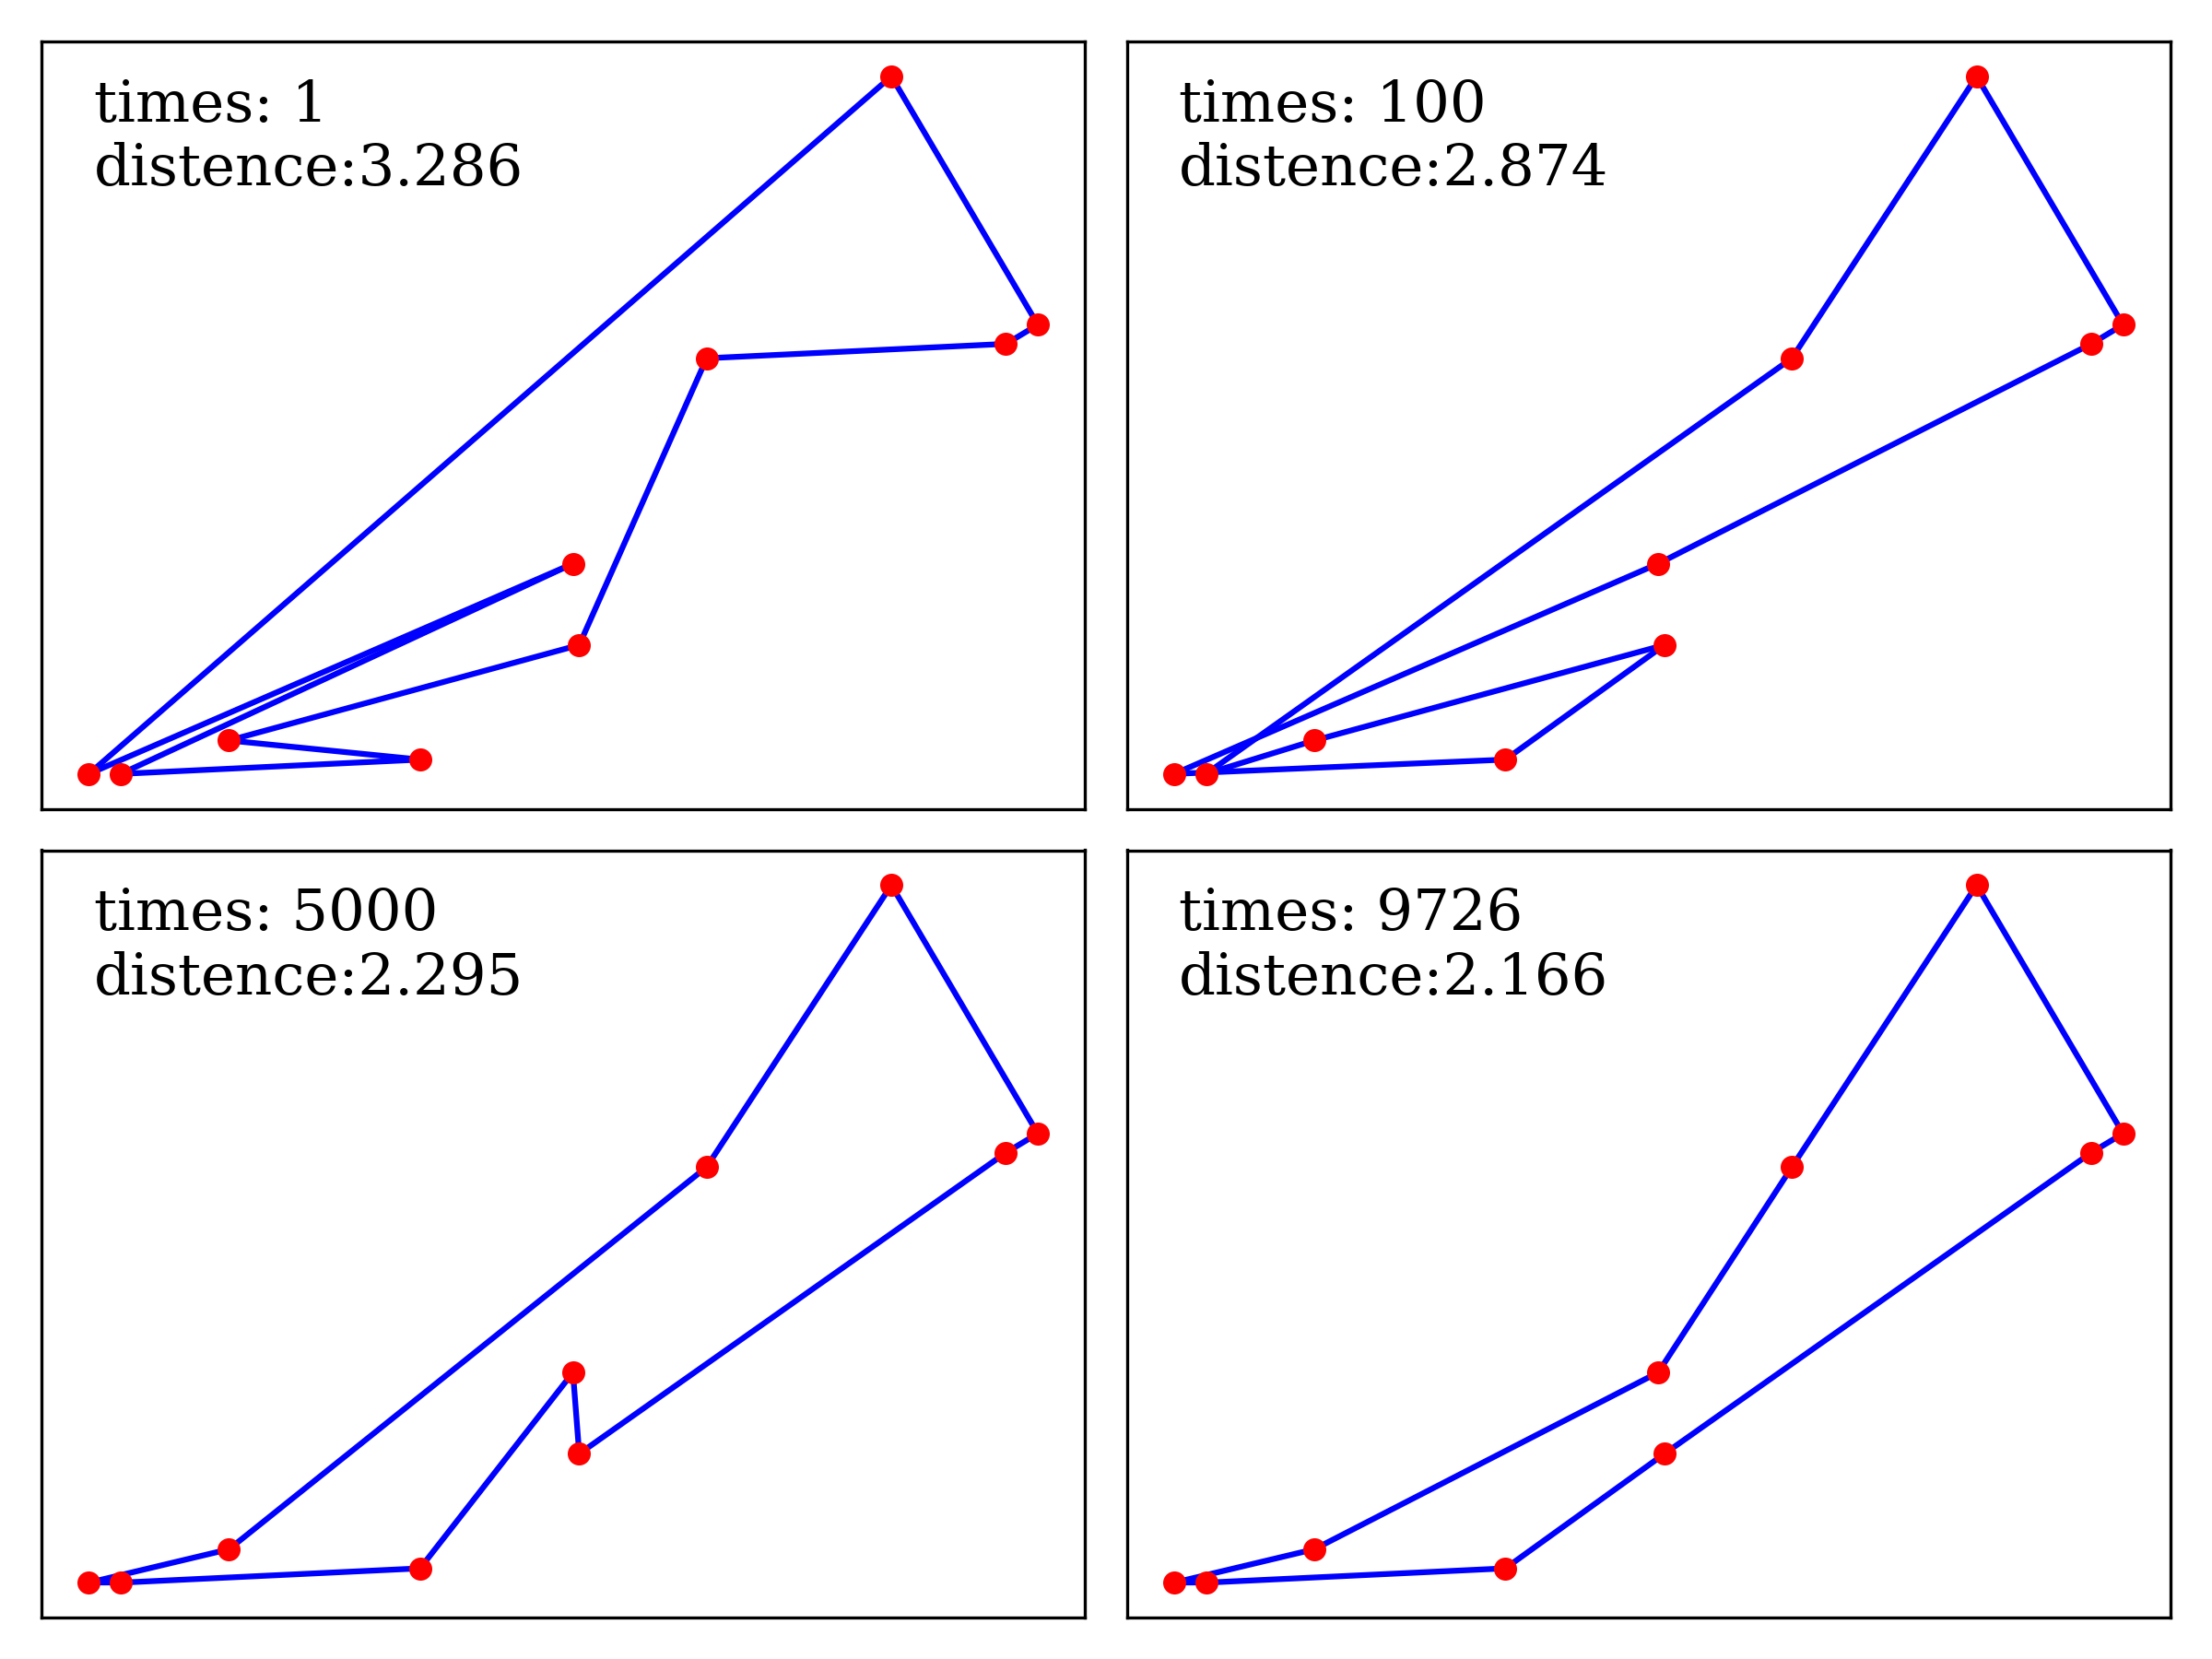
\includegraphics[scale=0.6]{simulated_annealing/TSP.png}
\end{figure}

    固定初始温度,终止温度,衰减系数不变,修改$K=1,5,10,100$可得最终距离和$K$的关系如下:
\renewcommand\arraystretch{0.8} % 设置表格高度为原来的0.8倍
\begin{table}[!htbp] % table标准
    \centering % 表格居中
    \begin{tabular}{p{2cm}<{\centering}p{2cm}<{\centering}p{2cm}<{\centering}p{2cm}<{\centering}p{2cm}<{\centering}} % 设置表格宽度
    %\begin{tabular}{cccc}
        \toprule
        $K$ & 1 & 5 & 50 & 100 \\
        \midrule
        最优距离 & 2.166 & 2.166 & 2.183 & 2.170 \\
        \bottomrule
    \end{tabular}
\end{table}

\clearpage
完整代码如下:
\begin{pythoncode}
import numpy as np
from pathlib import Path
import matplotlib.pyplot as plt
plt.rcParams['font.family'] = ['serif']
PATH_FIGURE = Path(__file__).parent

np.random.seed(42)
rand = np.random.rand; randint = np.random.randint  # 重载随机函数名
citys = np.loadtxt(Path(__file__).parent.joinpath("data.txt"))  # 数据读入
n = citys.shape[0]
def getdis(path):
    dis = 0;
    for i in range(n):
        dis += np.sqrt(np.sum(np.power(citys[path[i]] - citys[path[(i+1)%n]], 2)))
    return dis
def plot(path, cnt, ax:plt.Axes):
    for i in range(n):
        x, y = citys[path[i],:], citys[path[(i+1)%n],:]
        ax.plot([x[0],y[0]], [x[1],y[1]], '-b')
    ax.plot(citys[:,0], citys[:,1], '.r', markersize=10)
    ax.text(0.15, 0.83, f"times: {cnt}\ndistence:{getdis(path):.4}", fontsize=15)
    ax.set_xticks([]); ax.set_yticks([])

fig, axs = plt.subplots(2, 2, figsize=(8, 6)); ax = iter(axs.reshape(-1))
T = 168.14; K = 1; delta = 0.999; cnt = 0
path = list(range(n)); now = getdis(path)
best = {'path': path.copy(), 'dis': now}
while T >= 0.01:
    r = rand(); path_ = path.copy()
    if r <= 1/3:
        a, b = randint(0, n, size=2)  # 交换a和b
        while b == a: b = randint(0, n)
        path[a], path[b] = path[b], path[a]
    elif r <= 2/3:  # 使[s,s+l)区间段逆序
        s, l = randint(0,n,size=2); l = min(l, n-s); path[s:s+l] = reversed(path[s:s+l])
    else:  # 将path[p]插入到位置q的前面
        p, q = randint(0,n,size=2); idx = path[p]
        path = path[0:p] + path[p+1:]
        path = path[0:q] + [idx] + path[q:]
    new = getdis(path)
    if np.exp((now - new)/(T*K)) > rand(): now = new
    else: path = path_
    if now < best['dis']: best['dis'] = now; best['path'] = path.copy()
    T *= delta; cnt += 1
    if cnt in [1, 100, 5000]: plot(best['path'], cnt, next(ax))
plot(best['path'], cnt, next(ax))
print(f"最优路径: {best['path']}, 长度: {best['dis']}")
fig.tight_layout()
fig.savefig(PATH_FIGURE.joinpath("TSP.png"), dpi=300); plt.show()
\end{pythoncode}
\end{solution}
\end{document}